
%%%%%%%%%%%%%%%%%%%%%%%%%%%%%%%%%%%%%%%%%%%%%%%%%%%%%%%%
%
% Copyright (c) 2003-2009 by University of Queensland
% Earth Systems Science Computational Center (ESSCC)
% http://www.uq.edu.au/esscc
%
% Primary Business: Queensland, Australia
% Licensed under the Open Software License version 3.0
% http://www.opensource.org/licenses/osl-3.0.php
%
%%%%%%%%%%%%%%%%%%%%%%%%%%%%%%%%%%%%%%%%%%%%%%%%%%%%%%%%

\section{Escript and Python Basics} \label{sec:escpybas}

The Python scripting language is a powerful and easy to learn environment with a wide variety of applications. \textit{Escript} has been developed as a packaged module for Python specifically to solve complex partial differential equations. As a result, all the conventions and programming syntax associated with Python are coherent with \ESCRIPT. If you are unfamiliar with Python, there are a large number of simple to advanced guides and tutorials availabe online. These texts should provide an introduction that is comprehensive enough for the use of \ESCRIPT. A handful of python tutorials have been listed below.
\begin{itemize}
\item This is a very crisp introduction \url{http://hetland.org/writing/instant-python.html}. It covers everthing you need to get started with \ESCRIPT.
\item A nice and easy to follow introduction: \url{http://www.sthurlow.com/python/}
\item Another crisp tutorial \url{http://www.zetcode.com/tutorials/pythontutorial/}. 
 \item A very comprehensive tutorial from the python authors: \url{http://www.python.org/doc/2.5.2/tut/tut.html}. It covers much more than what you will ever need for \ESCRIPT.
\item Another comprehensive tutorial: \url{http://www.tutorialspoint.com/python/index.htm}
\end{itemize} 

\subsection{The \modesys Library Tree}
The \verb esys  library tree has \textbf{3} main modules, \verb escript , \verb finley  and \verb pycad . 
\begin{enumerate}
\item \modescript  is the PDE solving module.
\item \modfinley is the discretisation tool and finite element package.
\item \modpycad  is a special development for creating irregular domains and models. That are easily interpretable by \esc . 
\end{enumerate}
Further explanations on each of these is available in the user guide or in the API documentation at \url{https://launchpad.net/escript-finley/+download}. \ESCRIPT is also dependent on a few other open-source packages which are not maintained by the \ESCRIPT development team. These are \modnumpy an array and matrix handling package, \modmpl a simple plotting and visualisation tool, \modvtk  the advanced plotting and visualisation package and \verb gmsh  which is required by \modpycad. These packages (\textbf{except} for \verb gmsh ) are included with the binary release but may not be the most recent and up to date. 

\subsection{The Domain Constructor in \ESCRIPT}
\label{ss:domcon}
It is important at this paticular stage to describe how domains and data are organised and related to each other in escript.
\begin{figure}[t]
 \centering
   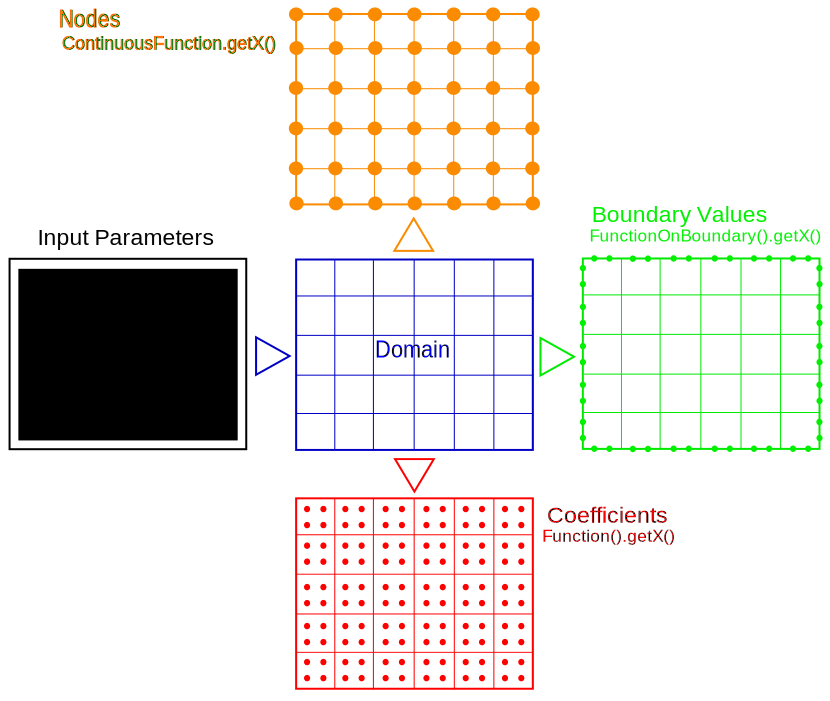
\includegraphics[width=4in]{figures/functionspace}
   \label{fig:fs}
   \caption{\ESCRIPT domain construction overview}
\end{figure}
When the domain variables are submitted to the domain constructor or meshing algorithm, three function spaces are also created. They are;
\begin{enumerate}
\item the nodes, called by \verb|ContinuousFunction(domain)| ;
\item the elements/coefficients, called by \verb|Function(domain)| ; and
\item the boundary, called by \verb|FunctionOnBoundary(domain)| .
\end{enumerate}
Domains in \ESCRIPT are constructed this way to allow for varying degrees of smoothness in a PDE problem. That is, the continuity of the first derivative of each data input. For example, the coefficients of a PDE need not be continuous, thus this qualifies as a \verb Function()  type, while a temperature distribution must be a \verb ContinuousFunction()  and a flux condition may only exist at a boundary as a \verb FunctionOnBoundary()  .  The domain constructor is able to interpret the data in each of these situations for the solver so that a solution can be produced. It should be noted that a solution has its own function space \verb Solution()  which is located depending on the required output. The domain also allows certain transformations of the function spaces. A \verb ContinuousFunction()  can be transformed into a \verb FunctionOnBoundary()  or \verb Function() . On the other hand there is not enough information in a \verb FunctionOnBoundary()  to transform it to a \verb ContinuousFunction()  .

The domain also handles an ability of \ESCRIPT known as tagging which allows areas and lines to be given a name for easier referencing later on. 

\subsection{File Commands and Operations in \ESCRIPT}
A number of common file operations and commands are used throughout this cookbook. It is often advantageous to implement these commands when large numbers of output files are generated or dependencies are located in other locations.

To develop an incrementing file name we can use the following convention. For this example we are going to use the \verb|os.path.join| command to join a subdirectory which already exists with the file name which we want to use for our output. The command is; 
\begin{verbatim}
os.path.join(save_path, "data%03d.xml"%i )
\end{verbatim}
There are two arguments to the \verb join  command. The \verb save_path  variable is a predefined string pointing to the directory we want to save our data in, for example a single subfolder called \verb data  would be defined by;
\begin{verbatim}
save_path = "data"
\end{verbatim}
while a subfolder of \verb data  called \verb ans_one  would be defined by;
\begin{verbatim}
save_path = "data/ans_one"
\end{verbatim}
The second argument of \verb join \xspace contains a string which is the filename. We can use the operator \verb|%| to increment our file names with the value \verb|i| our incrementing counter. The substring \verb %03d  does this by defining the following parameters; 
\begin{itemize}
 \item \verb 0  becomes the padding number;
 \item \verb 3  tells us the amount of padding numbers that are required; and
 \item \verb d  indicates the end of the \verb %  operator.
\end{itemize}
To increment the file name a \verb %i  is required directly after the operation the string is involved in. When correctly implemented the output files from this command would be place in the directory defined by \verb save_path  as;
\begin{verbatim}
data001.xml
data002.xml
data003.xml
...
\end{verbatim}
and so on.

A subfolder check/constructur is available in the cookbook \verb cblib  library called \verb needdirs . The command;
\begin{verbatim}
needdirs(save_path)
\end{verbatim}
will check for the existence of \verb save_path  and if needed, make the required directories.


\subsection{Visualisation and Plotting}
\ESCRIPT does not include its own plotting capabilities however it works with a number of free visualisation systems.
We will dicsuss two types of systems in this document: \mpl\footnote{\url{http://matplotlib.sourceforge.net/}} and \verb VTK \footnote{\url{http://www.vtk.org/}} visualisation. 
The \mpl package is based on the \numpy array package and is good for basic graphs and plots. The \verb VTK  toolkit allows the \esc data to be exported in a standardised format with powerful visualisation capabilities. This format can be interpreted by many programs. In this cookbook \mayavi \footnote{\url{http://code.enthought.com/projects/mayavi/}} will be used to visualise \verb VTK  files. 